\chapter{Homology}
\section{Complexes and homology}
\subsection{Complexes and exact sequences}
\begin{definition}
A \textbf{chain complex} $C_{\bullet}$ of $R$-modules is a family $\{C_n\}_{n\in\Z}$ of $R$-modules, together with $R$-module maps $d=d_n:C_n\to C_{n-1}$ such that each composite $d\circ d:C_n\to C_{n-2}$ is zero. The maps $d_n$ are called the \textbf{differentials} of $C_{\bullet}$. The kernel of $d_n$ is the module of $n$-cycles of $C_{\bullet}$, denoted $Z_n=Z_n(C_{\bullet})$. The image of $d_{n+1}:C_{n+1}\to C_n$ is the module of \textbf{$\bm{n}$-boundaries} of $C$, denoted $B_n=Bn(C_{\bullet})$. Because $d\circ d=0$, we have
\[0\sub B_n\sub Z_n\sub C_n\]
for all $n$. The $n$-th \textbf{homology} module of $C_{\bullet}$ is the subquotient $H_n(C_{\bullet})=Z_n/B_n$ of $C_n$.
\end{definition}
\begin{definition}
The category $\mathcal{C}(\mathcal{A})$ of chain complexes. The objects are chain complexes. A morphism $f:C_{\bullet}\to D_{\bullet}$ is a chain complex map, that is, a family of $R$-module homomorphisms $f_n:C_n\to D_n$ commuting with $d$ in the sense that $f_{n-1}\circ d_n=d_{n-1}f_n$. That is, such that the following diagram commutes:
\[\begin{tikzcd}
\cdots\ar[r,"d"]&C_{n+1}\ar[d,"f"]\ar[r,"d"]&C_n\ar[d,"f"]\ar[r,"d"]&C_{n-1}\ar[d,"f"]\ar[r,"d"]&\cdots\\
\cdots\ar[r,"d"]&D_{n+1}\ar[r,"d"]&C_n\ar[r,"d"]&C_{n-1}\ar[r,"d"]&\cdots\\
\end{tikzcd}\]
\end{definition}
\begin{definition}
A morphism $C_{\bullet}\to D_{\bullet}$ of chain complexes is called a \textbf{quasi-isomorphism} $($Bourbaki uses homologism$)$ if the induced maps $H_n(C_{\bullet})\to H_n(C_{\bullet})$ are all isomorphisms.
\end{definition}
It is sometimes useful to break up every exact complex into a large number of short exact
sequences:
\[\begin{tikzcd}[column sep=small, row sep=small]
&&0\ar[rdd]&&0&&\\
&&&&&&\\
&&&\im d_{i+1}=\ker d_i\ar[ruu]\ar[rdd]&&&\\
&&&&&&\\
M_{i+2}\ar[rdd]\ar[rr,"d_{i+2}"]&&M_{i+1}\ar[ruu]\ar[rr,"d_{i+1}"]&&M_{i}\ar[rdd]\ar[rr,"d_{i}"]&&M_{i-1}\\
&&&&&&\\
&\im d_{i+2}=\ker d_{i+1}\ar[rdd]\ar[ruu]&&&&\im d_i=\ker d_{i-1}\ar[rdd]\ar[ruu]&\\
&&&&&&\\
0\ar[ruu]&&0&&0\ar[ruu]&&0
\end{tikzcd}\]
\subsection{Split exact sequences}
A particular case of short exact sequence arises by considering the second projection from a direct sum: $M_1\oplus M_2\to M_2$; there is then an exact sequence
\[\begin{tikzcd}
0\ar[r]&M_1\ar[r]&M_1\oplus M_2\ar[r]&M_2\ar[r]&0
\end{tikzcd}\]
These short exact sequences are said to \textbf{split}; more generally, a short exact sequence
\[\begin{tikzcd}
0\ar[r]&M_1\ar[r]&N\ar[r]&M_2\ar[r]&0
\end{tikzcd}\]
is said to be exact if it is isomorphic to one of these sequences in the sense that there is a
commutative diagram
\[\begin{tikzcd}
0\ar[r]&M_1\ar[d,"\sim"]\ar[r]&N\ar[r]\ar[d,"\sim"]&M_2\ar[r]\ar[d,"\sim"]&0\\
0\ar[r]&M'_1\ar[r]&M'_1\oplus M'_2\ar[r]&M'_2\ar[r]&0
\end{tikzcd}\]
\begin{theorem}\label{split theo}
Let $\varphi:M\to N$ be an $R$-module homomorphism. Then
\begin{itemize}
\item $\varphi$ has a left-inverse if and only if the sequence
\[\begin{tikzcd}
0\ar[r]&M\ar[r,"\varphi"]&N\ar[r]&\coker\varphi\ar[r]&0
\end{tikzcd}\]
splits.
\item $\varphi$ has a right-inverse if and only if the sequence
\[\begin{tikzcd}
0\ar[r]&\ker\varphi\ar[r]&M\ar[r,"\varphi"]&N\ar[r]&0
\end{tikzcd}\]
\end{itemize}
\end{theorem}
\begin{proof}
If the sequence splits, then $\varphi$ may be identified with the embedding of $M$ into a direct sum $M\oplus M'$, and the projection $M\oplus M'\to M$ gives a left-inverse of $\varphi$. Conversely, assume that $\varphi$ has a left-inverse $\psi$:
\[\begin{tikzcd}
0\ar[r]&M\ar[r,"\varphi"]\ar[rd,"id"]&N\ar[d,"\psi"]\\
&&M
\end{tikzcd}\]
Then we claim that $N$ is isomorphic to $M\oplus\ker\psi$ and that $\varphi$ corresponds to the
identification of $M$ with the first factor: $M\to M\oplus\ker\psi\simeq N$. The isomorphism
$M\oplus\ker\psi\to N$ is given by
\[(m,k)\mapsto\varphi(m)+k\]
its inverse $N\to M\oplus\ker\psi$ is
\[n\mapsto(\psi(n),n-\varphi\psi(n))\]
The element $n-\varphi\psi(n)$ is in $\ker\psi$ as it should be, since
\[\psi(n-\varphi\psi(n))=\psi(n)-\psi\varphi\psi(n)=\psi(n)-\psi(n)=0\]
\end{proof}
Because of Proposition~\ref{split theo}, $R$-module homomorphisms with a left-inverse are called \textbf{split monomorphisms}, and homomorphisms with a right-inverse are called \textbf{split epimorphisms}.
\subsection{The snake lemma}
We begin with routine comments . Consider a commutative diagram of homomorphisms of modules.
\[\begin{tikzcd}
M'\ar[d,swap,"d'"]\ar[r,"f"]&M\ar[d,"d"]\\
N'\ar[r,"g"]&N
\end{tikzcd}\]
Then $f$ induces a homomorphism
\[\ker d'\to\ker d\]
Indeed, suppose $d'(m')=0$. Then $df(m')=0$ because $df(m')=gd'(m')=0$.\par
Similarly, $g$ induces a homomorphism
\[\coker d'\to\coker d\]
in a natural way as follows. Let $n'\in N'$ represent an element of $\coker d'=N'/\im d'$. Then $g(n')$ mod $\im d'$ does not depend on the choice of $n'$ representing the given element, because if $n''=n'+d'(m')$, then
\[g(n'')=g(n')+gd'(m')=g(n')+df(m')\equiv g(n')\mod \im d\]
Thus we get a map
\[g_*:\coker d'\to\coker d\]
which is immediately verified to be a homomorphism.\par
In practice , given a commutative diagram as above , one sometimes writes $f$ instead of $g$, so one writes $f$ for the horizontal maps both above and below the diagram. This simplifies the notation, and is not so incorrect: we may view $M'$, $N'$ as the two components of a direct sum, and similarly for $M, N$. Then $f$ is merely a homomorphism defined on the direct sum $M'\oplus N'$ into $M\oplus N$.\par
\begin{lemma}[\textbf{snake lemma}]\label{snake lemma}
If given a \textbf{snake diagram} as follows
\[\begin{tikzcd}
&A\ar[r,"f"]\ar[d,"\alpha"]&B\ar[r,"g"]\ar[d,"\beta"]&C\ar[r]\ar[d,"\gamma"]&0\\
0\ar[r]&A'\ar[r,"f'"]&B'\ar[r,"g'"]&C'
\end{tikzcd}\]
where the two rows are exact. Then there is an homomorphism $\delta:\ker\gamma\to\coker\alpha$ such that the follows diagram commutes
\begin{figure}[!h]
\centering
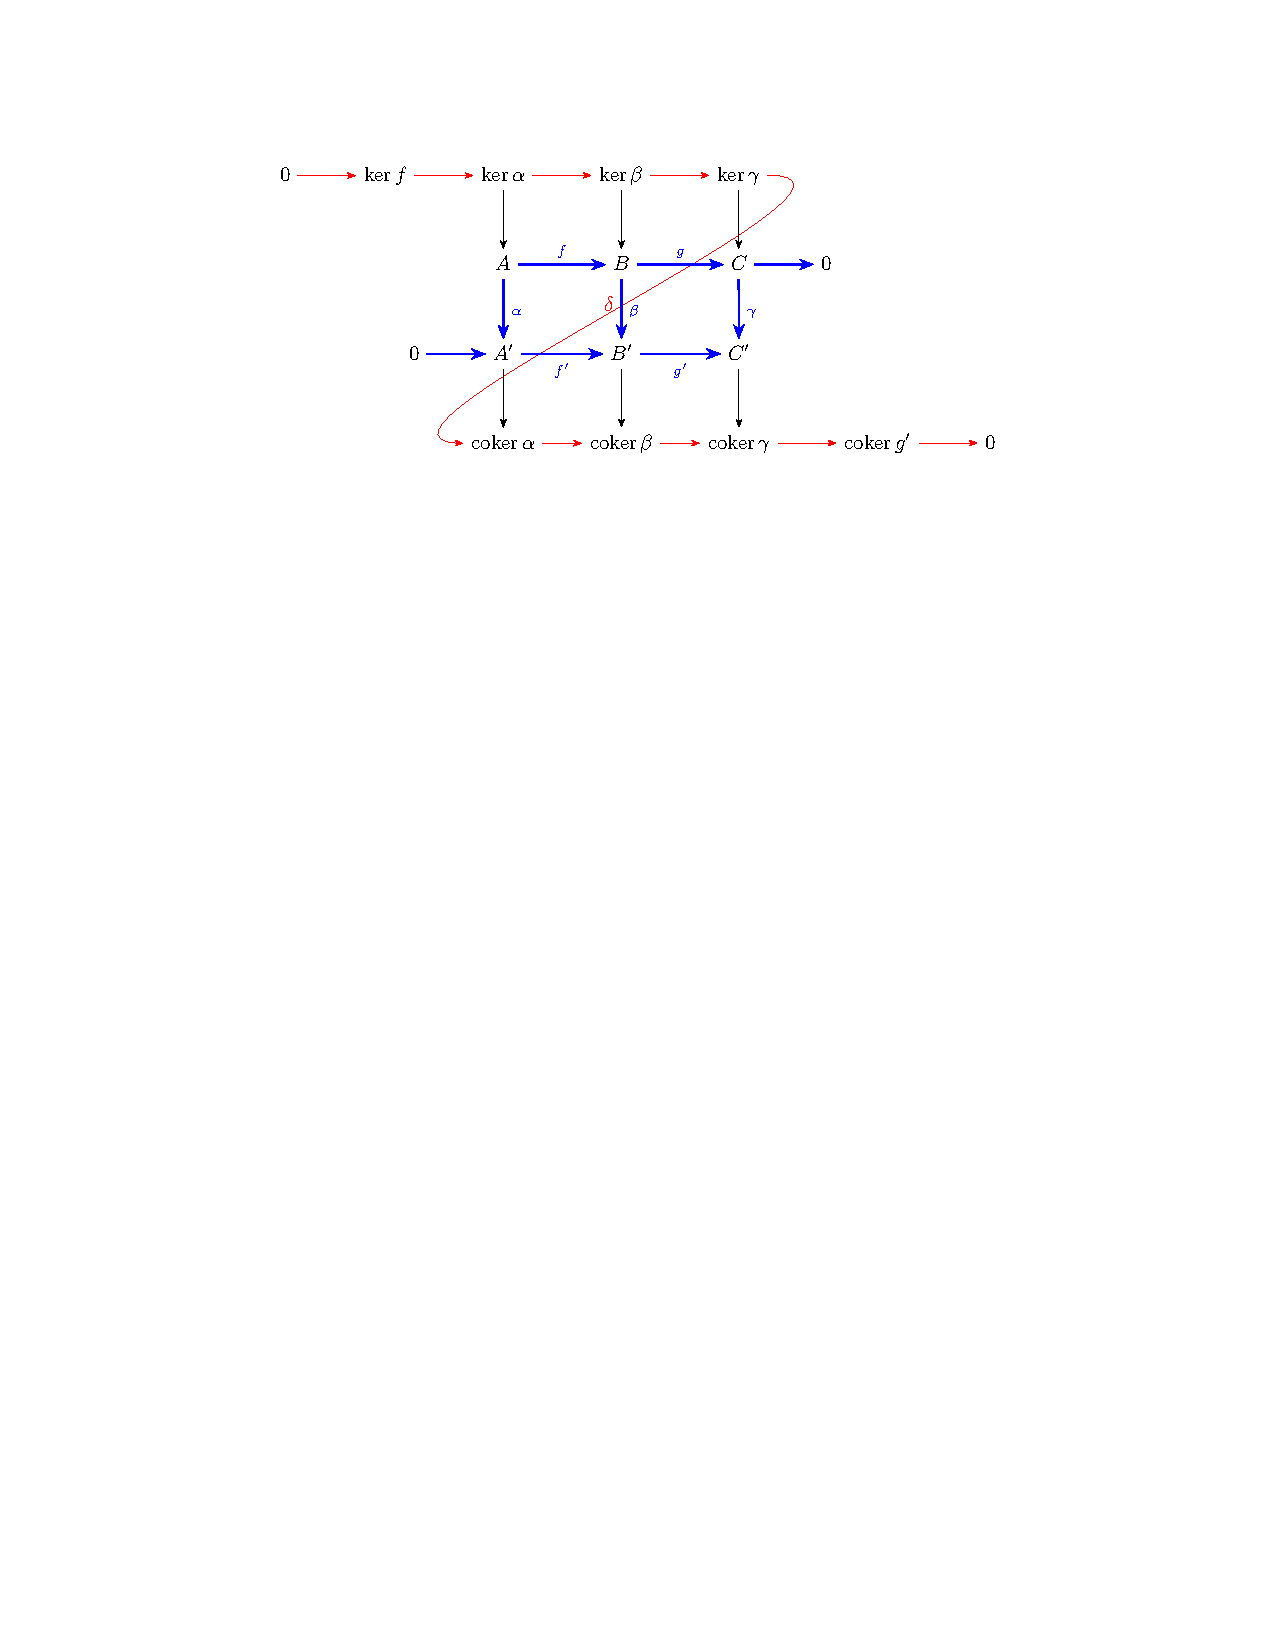
\includegraphics{pictures/snake.pdf}
\end{figure}
the homomorphism $\delta$ is called the \textbf{connection homomorphism}.
\end{lemma}
\begin{proof}
First, let $c\in\ker\gamma$, We can construct elements of $A'$ as follows. 
\begin{itemize}
\item Since $g$ is surjective, there exists an element $b\in B$ such that $g(b)=c$. We now move vertically down by $\beta$, and take $\beta(b)$.
\item The commutativity $\gamma\circ g=g'\circ\beta$ shows that 
\[g'(\beta(b))=\gamma(g(b))=\gamma(c)=0\]
whence $\beta(b)$ is in the kernel of $g'$ in $B'$. By exactness, there exists an element $a'\in A'$ such that $f'(a)=\beta(b)$. We map $a$ into $\coker\alpha$ by the canonical projection, and still denote it by $a$.
\end{itemize}
In brief, we write
\[\delta(c)=a=f'^{-1}\circ\beta\circ g^{-1}(c)\]
\[\begin{tikzcd}
&&c\ar[d]\\
&b\ar[d,"\beta"]\ar[r,"g"]&c\ar[d,dashed,"\gamma"]\\
a\ar[d]\ar[r,"f'"]&\beta(b)\ar[r,dashed,"g'"]&0\\
a&&
\end{tikzcd}\]
\newline
We now verify that $\delta$ is well defined. First, $f'$ is injective by exactness, $a$ is uniquely determined by $\beta(b)$, hence by $b$. So the only verification is for $b$.\par
\begin{itemize}
\item Suppose we choose a different $b'$ mapping to the same $c$: $g(b')=c=g(b)$. Then $b'-b\in\ker g$, and by exactness, $\im f=\ker g$, so there is $\ell\in A$ such that $\alpha(\ell)=b'-b$.
\item It follows from the commutativity that
\[\beta(b'-b)=\beta(f(b'-b))=f'(\alpha(\ell))\]
Following our construction, $f'^{-1}(\beta(b'-b))=\alpha(\ell)$. But since the column is exact, the projection into $\coker\alpha$ kills $\alpha(\ell)$, hence taking $b'$ makes no difference to $\delta(c)$, that is, $\delta$ is well defined.
\[\begin{tikzcd}
\ell\ar[d,"\alpha"]\ar[r,"f"]&b'-b\ar[d,"\beta"]\ar[r,"g"]&0\\
\alpha(\ell)\ar[d]\ar[r,"f'"]&\beta(b'-b)&\\
0&&
\end{tikzcd}\]
\end{itemize}
The rest part is rather easy, we need to verify the exactness of the sequence. First we give the morphisms in the sequence
\[\begin{tikzcd}[column sep=tiny]
0\ar[r]&\ker f\ar[r,"i"]&\ker\alpha\ar[r,"f_*"]&\ker\beta\ar[r,"g_*"]&\ker\gamma\ar[r,"\delta"]&\coker\alpha\ar[r,"f'_*"]&\coker\beta\ar[r,"g'_*"]&\coker\gamma\ar[r,"j"]&\coker g'\ar[r]&0
\end{tikzcd}\]
We just define $f_*:=f|_{\ker\alpha}$, and similar for $g_*$, $f'_*,g'_*$.\par
If $a\in\ker f$, then $f'(\alpha(a))=0$ by commutativity, and $\alpha(a)=0$ by injectvity of $f'$. This gives an inclusion $\ker f\to\ker\alpha$, which is our $i$.\par
Similarly, if $c\in\im\gamma$, then there is an element $b\in B$ such that $\gamma(g(b))=c$ by the surjectivity of $g$. Then we see $c=g'(\beta(b))$ by commutativity, hence $c\in\im g'$. This gives $\im\gamma\sub\im g'$, and we have an induced quotient map $\coker\gamma\to\coker g'$. This is our $j$.\par
By our definition, the exactness of two ends follows, now we begin to verify the rest:
\begin{itemize}
\item Since $\ker f\sub\ker\alpha$, by our definition of $f_*$, the exactness at $\ker\alpha$ follows. Similar for the exactness of $\coker\gamma$.
\item  Since the top row is exact, $\im(f)=\ker(g)$. Ii follows that $g_*\circ f_*=0$, so $\im f_*\sub\ker g_*$. To verify the converse, assume $b\in\ker g_*$, that is, $b\in\ker\beta$ and $g(b)=0$. By exactness of $B$, there is $a\in A$ such that $f(a)=b$. We show that $a\in\ker\alpha$: in fact,
\[f'(\alpha(a))=\beta(f(a))=\beta(b)=0\]
Since $f'$ is injective, this means $\alpha(a)=0$, so $a\in\ker\alpha$. Thus $\ker g_*=\im f_*$, giving the exactness at $\ker\beta$.\par
The exactness at $\coker\beta$ arises similarly. Assume $b'+\im\beta\in\ker g'_*$, then $g'(b')\in\im\gamma$. By the surjectivity of $g$, $\exists b\in B$ such that $g'(b')=\gamma(g(b))=g'(\beta(b))$. Then $b'=\beta(b)+x$ with $x\in\ker g'$. By exactness, $x=f'(a')$ for some $a'\in A'$. Then it follows
\[b'+\im\gamma=\beta(b)+f'(a')+\im\beta=f'(a')\]
this shows $\ker g'_*\sub \im f'_*$, and the claim.
\item We verify the exactness about $\delta$. First, let $c=g(b)$ for some $b\in\ker\beta$. Since $\beta(b)=0$, by our definition of $\delta$, $\delta(c)=f'^{-1}(\beta(b))+\im\alpha=\im\alpha$. This gives $\im g_*\sub\ker\delta$. Conversely, if $\delta(c+\im\alpha)=\im\alpha$ for some $c\in C$, we get $\delta(c)\in\im\alpha$, hence $\delta(c)=\alpha(a)$ by some $a\in A$. By the construction of $\delta$, choose some $b\in B$ such that $g(b)=c$, then $f'^{-1}(\beta(b))=\delta(c)=\alpha(a)$ . It follows that
\[\beta(b)=f'(\alpha(a))=\beta(f(a))\]
and $b=f(a)+x$ for $x\in\ker\beta$. Applying $g$ we get $c=g(b)=g(f(a))+g(x)=g(x)$ since $g\circ f=0$. Since $x\in\ker\beta$, $g_*(x)=g(x)=c$. This gives $\ker\delta\sub\im g_*$, giving the exactness at $\ker\gamma$.
\item Finally, we deal with the exactness at $\coker\alpha$. Choose $a'+\im\alpha=\delta(c)$ for $c\in\ker\gamma$. Agian the definition of $\delta$: $f'(a')=f'(\delta(c))=\beta(b)$ for some $g(b)=c, b\in B$. This already gives 
\[f'_*(a'+\im\alpha)=f'(\delta(c))+\im\beta=\beta(b)+\im\beta=\im\beta\]
For the other direction, let $a'+\im\beta\in\ker f'_*$, that is, $f'(a')\in\im\beta$. So let $f'(a')=\beta(b), b\in B$, we observe that $a'=f'^{-1}\circ\beta(b)=f'^{-1}\circ\beta\circ g^{-1}(g(b))=\delta(g(b))$. This gives $\ker f'_*\sub\im\delta$, finishing the proof.
\end{itemize}
\end{proof}
\begin{corollary}
In the same situation presented in the snake lemma $($notation as in above$)$, assume that $\beta$ is surjective, $g'$ is surjective and $\gamma$ is injective. Then $\alpha$ is surjective and $\gamma$ is an isomorphism.
\end{corollary}
\begin{proof}
With the condition, the exact sequence
\[\begin{tikzcd}[column sep=tiny]
0\ar[r]&\ker f\ar[r]&\ker\alpha\ar[r]&\ker\beta\ar[r]&\ker\gamma\ar[r,"\delta"]&\coker\alpha\ar[r]&\coker\beta\ar[r]&\coker\gamma\ar[r]&\coker g'\ar[r]&0
\end{tikzcd}\]
becomes
\[\begin{tikzcd}[column sep=tiny]
0\ar[r]&\ker f\ar[r]&\ker\alpha\ar[r]&\ker\beta\ar[r]&0\ar[r,"\delta"]&\coker\alpha\ar[r]&0\ar[r]&\coker\gamma\ar[r]&0\ar[r]&0
\end{tikzcd}\]
the claim follows.
\end{proof}
\subsection{Exercise}
\begin{exercise}
Prove the \textbf{four lemma}: if
\[\begin{tikzcd}
A_1\ar[r]\ar[d,"\alpha"]&B_1\ar[d,"\beta"]\ar[r]&C_1\ar[d,"\gamma"]\ar[r]&D_1\ar[d,"\delta"]\\
A_0\ar[r]&B_0\ar[r]&C_0\ar[r]&D_0
\end{tikzcd}\]
is a commutative diagram of $R$-modules with exact rows, $\alpha$ is an epimorphism, and
$\beta$, $\delta$ are monomorphisms, then $\gamma$ is an monomorphism.
\end{exercise}
\begin{proof}
Write the morphisms:
\[\begin{tikzcd}
A_1\ar[r,"f_1"]\ar[d,"\alpha"]&B_1\ar[d,"\beta"]\ar[r,"g_1"]&C_1\ar[d,"\gamma"]\ar[r,"h_1"]&D_1\ar[d,"\delta"]\\
A_0\ar[r,"f_0"]&B_0\ar[r,"g_0"]&C_0\ar[r,"h_0"]&D_0
\end{tikzcd}\]
\item Suppose $\gamma(c)=0$ for $c\in C_1$, then $\delta\circ h_1(c)=0$, hence $h_1(c)=0$ since $\delta$ is a monomorphism. With $\ker h_1=\im g_1$, there is $b\in B_1$ such that $g_1(b)=c$. It follows that $g_0(\beta(b))=\gamma(g(b))=\gamma(c)=0$. Hence $\beta(b)\in\ker g_0$. From $\im f_0=\ker g_0$, there is $a\in A_0$ s.t. $f_0(a)=\beta(b)$. By the surjectivity of $\alpha$, there is $a'\in A_1$ with $\alpha(a')=a$. Then $\beta(b)=f_0(\alpha(a'))=\beta(f_1(a'))$, hence $b=f_1(a')$ since $\beta$ is an monomirphism. This gives $c=g_0(b)=g_1(f_1(a'))=0$, proving $\gamma$ is injective\par
\end{proof}
\begin{exercise}
Prove another version of the four-lemma: if
\[\begin{tikzcd}
B_1\ar[r]\ar[d,"\beta"]&C_1\ar[r]\ar[d,"\gamma"]&D_1\ar[r]\ar[d,"\delta"]&E_1\ar[d,"\epsilon"]\\
B_0\ar[r]&C_0\ar[r]&D_0\ar[r]&E_0
\end{tikzcd}\]
is a commutative diagram of $R$-modules with exact rows, $\beta$ and $\delta$ are epimorphisms, and $\epsilon$ is a monomorphism, then $\gamma$ is an epimorphism.
\end{exercise}
\begin{proof}
\[\begin{tikzcd}
B_1\ar[r,"f_1"]\ar[d,"\beta"]&C_1\ar[r,"g_1"]\ar[d,"\gamma"]&D_1\ar[r,"h_1"]\ar[d,"\delta"]&E_1\ar[d,"\epsilon"]\\
B_0\ar[r,"f_0"]&C_0\ar[r,"g_0"]&D_0\ar[r,"h_0"]&E_0
\end{tikzcd}\]
Take $c\in C_0$, since $\delta$ is epimorphic, there is $d\in D_1$ such that $\delta(d)=g_0(c)$. Since $h_0(\delta(d))=0$, by the commutativity, $\epsilon(h_1(d))=0$. While $\epsilon$ is a monomorphism, so $h_1(d)=0$, then $d\in\ker h_1=\im g_1$. It follows that $d=g_1(c')$ for some $c'\in C_1$. Hence we have
\[g_0(c)=\delta(d)=\delta(g_1(c'))=g_0(\gamma(c'))\]
and $c=\gamma(c')+x$ with $x\in\ker g_0=\im f_0$. With the fact that $\beta$ is a epimorphism, $f_0(\beta(b))=x$ for some $b\in B_1$. Since $f_0(\beta(b))=\gamma(f_1(b))$, we have $x\in\im\gamma$, so $c\in\im\gamma$ follows.
\end{proof}
\begin{exercise}\label{nine lemma}
Consider the following commutative diagram of $R$-modules:
\[\begin{tikzcd}
&0\ar[d] &0\ar[d] &0\ar[d]\\
0\ar[r]&L_2\ar[d]\ar[r]&M_2\ar[r]\ar[d,"\alpha"]&N_2\ar[r]\ar[d]&0\\
0\ar[r]&L_1\ar[d]\ar[r]&M_1\ar[r]\ar[d,"\beta"]&N_1\ar[r]\ar[d]&0\\
0\ar[r]&L_0\ar[d]\ar[r]&M_0\ar[r]\ar[d]&N_0\ar[r]\ar[d]&0\\
&0&0&0
\end{tikzcd}\]
Assume that the three rows are exact and the two rightmost columns are exact. Prove that the left column is exact. Second version: assume that the three rows are exact and the two leftmost columns are exact; prove that the right column is exact. This is the \textbf{nine-lemma}.
\end{exercise}
\begin{proof}
For the first, since the rows are exact, we can write
\[\begin{tikzcd}
&0\ar[d] &0\ar[d] &0\ar[d]\\
0\ar[r]&\ker f\ar[d]\ar[r]&M_2\ar[r,"f"]\ar[d,"\alpha"]&N_2\ar[r]\ar[d]&0\\
0\ar[r]&\ker g\ar[d]\ar[r]&M_1\ar[r,"g"]\ar[d,"\beta"]&N_1\ar[r]\ar[d]&0\\
0\ar[r]&\ker h\ar[d]\ar[r]&M_0\ar[r,"h"]\ar[d]&N_0\ar[r]\ar[d]&0\\
&0&0&0
\end{tikzcd}\]
now apply snake lemma to the sequence
\[\begin{tikzcd}
0\ar[r]&M_2\ar[d]\ar[r]&M_1\ar[d]\ar[r]&M_0\ar[d]\ar[r]&0\\
0\ar[r]&N_2\ar[r]&N_1\ar[r]&N_0\ar[r]&0\\
\end{tikzcd}\]
we get the claim.\par
We write
\[\begin{tikzcd}
&0\ar[d] &0\ar[d] &0\ar[d]\\
0\ar[r]&L_2\ar[d]\ar[r,"f"]&M_2\ar[r]\ar[d,"\alpha"]&\coker f\ar[r]\ar[d]&0\\
0\ar[r]&L_1\ar[d]\ar[r,"g"]&M_1\ar[r]\ar[d,"\beta"]&\coker g\ar[r]\ar[d]&0\\
0\ar[r]&L_0\ar[d]\ar[r,"h"]&M_0\ar[r]\ar[d]&\coker h\ar[r]\ar[d]&0\\
&0&0&0
\end{tikzcd}\]
applying snake lemma gives the claim.
\end{proof}
\begin{exercise}
In the same situation as in Exercise~\ref{nine lemma}, assume that the three rows are
exact and that the leftmost and rightmost columns are exact.
\begin{itemize}
\item Prove that $\alpha$ is a monomorphism and $\beta$ is an epimorphism.
\item Is the central column necessarily exact?
\item Assume further that the central column is a complex $($that is, $\beta\circ\alpha=0$$)$; prove that it is then necessarily exact.
\end{itemize}
\end{exercise}
\begin{proof}
\mbox{}
\begin{itemize}
\item $\alpha$ is monic: If $m_2\in M_2$ maps to $0$ in $M_1$, it maps to $0$ in $N_1$, hence maps $0$ in $N_2$ since $N_2\to N_2$ is monic. Then there is a $l_2\in L_2$ maps to $m_2$. Since $l_2$ maps to $0$ in $M_1$, and $L_2\to L_1\to M_1$ is monic, it follows $l_2=0$, hence $m_2=0$.
\item $\beta$ is epic: take $m_0\in M_0$, map it to $n_0\in N_0$, since $N_1\to N_0$, $M_1\to N_1$ is epic, $n_0$ has a preimage $m_1\in M_1$. Let $m_1'$ be its image in $M_0$. Then by commutativity $m_1'-m_0$ maps to $0$ in $N_0$, hence has a preimage in $L_0$, and preimage $l_1$ in $L_1$. Then $M_1'-m_0$ is in the image of $\beta$, by the commutativity. It follows that $m_0\in\im\beta$.
\item If $\beta\circ\alpha=0$, then $\ker\beta\sub\im\alpha$: let $m_1$ maps to $0$ in $M_0$ by $\beta$, consider its image $n_1\in N_1$. $n_1$ maps $0$ to $N_0$, hence has a preimage $n_2\in N_2$, and preimage $m_2$ in $M_2$. By commutativity, $\alpha(m_2)-m_1$ is maped to $0$ in $N_1$, so has a preimage $l_1$ in $L_1$. Here we use $\beta\circ\alpha=0$, $\alpha(m_2)-m_1$ is send to $0$ in $M_0$ by $\beta$, hence so does $l_1$. Snce $L_0\to M_0$ is monic, $l_1$ maps to $0$ in $L_0$. Then $l_1$ has a preimage $l_2$ in $L_2$. It follows that $l_2$ maps to $\alpha(m_2)-m_1$, hence $\alpha(m_2)-m_1\in\im\alpha$. Now it follows $m_1\in\im\alpha$. The other direction follows easily from $\beta\circ\alpha=0$. Hence the colum is exact in this case.
\item Counterexample:
\[\begin{tikzcd}
0\ar[d]\ar[r]&R\ar[d,"{(id,0)}"]\ar[r,"id"]&R\ar[d,"id"]\\
R\ar[d]\ar[r,"{(id,id)}"]&R\oplus R\ar[d,"{(id,0)}"]\ar[r,"{(id,-id)}"]&R\ar[d]\\
R\ar[r,"id"]&R\ar[r]&0
\end{tikzcd}\]
\end{itemize}
\end{proof}
\section{Relative Homology}
For a map $f:X\to Y$, a induced homomorphism: $f_\sharp:C_n(X)\to C_n(Y)$ is defined as
\[f_\sharp(\sum_i n_i\sigma_i)=\sum_i n_if_\sharp\sigma_i\]
And we have $f_\sharp\partial=\partial f_\sharp$, since
\[f_\sharp\partial(\sigma)=f_\sharp(\sum_i (-1)^{i}\sigma|[v_0,\cdots,\hat{v_i},\cdots,v_n])=\sum_i(-1)^if\sigma|[v_0,\cdots,\hat{v_i},\cdots,v_n]=\partial f_\sharp(\sigma)\]
we have the diagram
\[\begin{tikzcd}
\cdots\arrow{r} 
&C_{n+1}(X)\arrow[r,"\partial"] \arrow[d,"f_\sharp"]
&C_n(X)\arrow[r,"\partial"]\arrow[d,"f_\sharp"]
&C_{n-1}(X)\arrow[r]\arrow[d,"f_\sharp"]
&\cdots\\
\cdots\arrow[r]
&C_{n+1}(Y)\arrow[r,"\partial"] 
&C_n(Y)\arrow[r,"\partial"]
&C_{n-1}(Y)\arrow[r] 
&\cdots
\end{tikzcd}
\]

\begin{itemize}
	\item $\partial\alpha=0\Rightarrow\partial(f_\sharp\alpha)=f_\sharp(\partial\alpha)=0$\quad (cycle to cycle)
	\item $\partial(f_\sharp\beta)=f_\sharp(\partial\beta)$\quad (boundary to boundary)
	
\end{itemize}
so $f_\sharp$ induces a homomorphism $f_*:H_n(X)\to H_n(Y)$.
\begin{proposition}[Functorial Property]
	A chain map between chain complexes induces homomorphisms between the homology groups of them, and we have the funtorial properties:
	\begin{itemize}
		\item[$(\rmnum{1})$] $(fg)_*=f_*g_*$ 
		\item[$(\rmnum{2})$] $id_*=id$
	\end{itemize}
	\end{proposition}
This shows that the homology group is a functor between the category $\mathfrak{Tpo}$ to the category $\mathfrak{Grp}$. Hence it preserves isomorphisms.
\vspace{5mm}
\begin{theorem}
	If $X$ is a space and A is a nonempty closed subspace that is a deformation retract of some neighborhood in X, then there is a exact sequence
\[
\begin{tikzcd}[cramped]
	\cdots \ar[r," "] &H_n(A)\ar[r,"i_*"] &H_n(X) \ar[r,"j_*"] &H_n(X/A) \ar[r,"\delta"] &H_{n-1}(A) \ar[r,"i_*"]&\cdots
\end{tikzcd}
\]
where $i$ is the inclusion $A\hookrightarrow X$ and $h$ is the quotient map $X\to X/A$.
\end{theorem}
We will prove a general one, which holds for arbitrary pairs.
\begin{definition}
Given a space X and a subspace $A\sub X$, let $C_n(X,A)=C_n(X)/C_n(A)$. Thus chains in A are trivial in $C_n(X,A)$. Since the boundary map $\partial_n: C_n(X)\to C_{n-1}(X)$ takes $C_n(A)$ to $C_{n-1}(A)$, it induces a quotient boundary map:
\begin{equation*}
\begin{split}
&\ \partial_n: C_n(X,A)\longrightarrow C_{n-1}(X,A)\\
&\sigma+C_n(A)\longmapsto \partial_n(\sigma)+C_{n-1}(A)
\end{split}
\end{equation*}
The relation $\partial_n\circ\partial_{n+1}=0$ still holds. So we have a chain complex and we can define the homology groups:
\[H_n(X,A)=\dfrac{\ker\ \partial_n}{\im\ \partial_{n+1}}\]
\end{definition}
by considering the definition we see:
\begin{itemize}
	\item Elements of $H_n(X,A)$ are represented by \textbf{relative cycles}: n-chains $\alpha\in C_n(X)$ such that $\partial_n(\alpha)\in C_{n-1}(A)$, cause we have $\partial_n(\alpha)=0$ in $C_{n-1}(X,A)$.
	\item A relative cycle $\alpha$ is trivial in $H_n(X,A)$ iff it is a \textbf{relative boundary} : $\alpha=\partial_{n+1}(\beta)+\gamma$ for some $\beta\in C_{n+1}(X)$ and $\gamma\in C_n(A)$, cause we have
	\[\alpha\ \text{is trivial}\iff \alpha\in \im\ \partial_{n+1}\iff \exists\ \beta\in C_{n+1}(X,A),\ \partial_{n+1}(\beta)+C_{n}(A)=\alpha+C_n(A)\]
\end{itemize}
Now our goal is to show that the relative homology groups $H_n(X,A)$ for any pair $(X,A)$ fit into a long exact sequence 
\[
\begin{tikzcd}[cramped]
\cdots \ar[r," "] &H_n(A)\ar[r,"i_*"] &H_n(X) \ar[r,"j_*"] &H_n(X,A) \ar[r,"\delta"] &\tilde{H}_{n-1}(A) \ar[r,"i_*"]&\cdots
\end{tikzcd}
\]
\begin{theorem}
	For arbitrary pairs $(X,A)$, we have a long exact sequence of homology groups
	\[
	\begin{tikzcd}[cramped]
	\cdots \ar[r,] &H_n(A)\ar[r,"i_*"] &H_n(X) \ar[r,"j_*"] &H_n(X,A) \ar[r,"\delta"] &H_{n-1}(A) \ar[r,"i_*"]&\cdots
	\end{tikzcd}
	\]
\end{theorem}
\begin{proof}
	We have already many short exact sequences:
	\[\begin{tikzcd}
	0\ar[r]&C_n(A)\ar[r,"i"]\ar[d,"\partial_n"]&C_n(X)\ar[d,"\partial_n"]\ar[r,"j"]&C_{n}(X,A)\ar[d,"\partial_n"]\ar[r]&0\\
	0\ar[r]&C_{n-1}(A)\ar[r,"i"]&C_{n-1}(X)\ar[r,"j"]&C_{n-1}(X,A)\ar[r]&0
	\end{tikzcd}\]
this diagram is commutative form the definition of $\partial_n$.\\
To begin with, we draw the short exact sequences, forming into a large commutative diagram:
\[\begin{tikzcd}
&0\ar[d] &0\ar[d] &0\ar[d]\\
\cdots\ar[r] 
&A_{n+1}\ar[d,"i"] \ar[r,"\partial_{n+1}"] 
&A_n\ar[r,"\partial_{n}"] \ar[d,"i"]
&A_{n-1}\ar[r] \ar[d,"i"]
&\cdots\\
\cdots \ar[r]
& B_{n+1} \ar[r,"\partial_{n+1}"]\ar[d,"j"]
& B_n \ar[r,"\partial_{n}"] \ar[d,"j"]
& B_{n-1}\ar[r] \ar[d,"j"]
&\cdots\\
\cdots \ar[r]
& C_{n+1} \ar[r,"\partial_{n+1}"]\ar[d]
& C_n \ar[r,"\partial_{n}"] \ar[d]
& C_{n-1}\ar[r] \ar[d]
&\cdots\\
&0 &0 &0
\end{tikzcd}\]
we will show that we can get a long exact sequence:
	\[
\begin{tikzcd}[cramped]
\cdots \ar[r,] &H_n(A)\ar[r,"i_*"] &H_n(B) \ar[r,"j_*"] &H_n(C) \ar[r,"\delta"] &H_{n-1}(A) \ar[r,"i_*"]&\cdots
\end{tikzcd}
\]
\newline
The commutativity of $i$ and $j$ show that they are chain maps, hence they induce maps $i_*$ and $j_*$ on homology groups.\\
Now we define the boundary map $\delta: H_n(C)\to H_{n-1}(A)$. \\
Let $c$ be a cycle, which is to say $c\in C_n$ and $\partial_n(c)=0$.\\
\begin{tikzcd}
&0 \ar[d] &0 \ar[d] &0 \ar[d] &0 \ar[d]\\
\cdots \ar[r] 
&A_{n+1} \ar[d,"i"] \ar[r,"\partial_{n+1}"] 
&A_n \ar[r,"\partial_{n}"] \ar[d,"i"]
&A_{n-1} \ar[r,"\partial_{n-1}"] \ar[d,"i"]
&A_{n-2} \ar[r] \ar[d,"i"]
&\cdots\\
\cdots \ar[r]
& B_{n+1} \ar[r,"\partial_{n+1}"]\ar[d,"j"]
& B_n \ar[red,r,"\partial_{n}",dashed] \ar[d,"j"]
& B_{n-1} \ar[r,"\partial_{n-1}"] \ar[d,"j"] \ar[u,red,dashed,shift left=1.0ex]
& B_{n-2} \ar[r] \ar[d,"i"]
&\cdots\\
\cdots \ar[r]
& C_{n+1} \ar[r,"\partial_{n+1}"] \ar[d] 
& C_n \ar[r,"\partial_{n}"] \ar[d] \ar[u,red,dashed,shift left=1.0ex]
& C_{n-1} \ar[r,"\partial_{n-1}"] \ar[d]
& C_{n-2} \ar[r] \ar[d]
&\cdots\\
&0 &0 &0 &0
\end{tikzcd}
\begin{tikzcd}[cramped, column sep=small]
&              &a\\
&b \ar[r]      &\partial_n(b) \ar[u]\\
&c \ar[u]
\end{tikzcd}
\begin{tikzcd}[cramped,column sep=small]
&              &A_{n-1}\\
&B_n \ar[r]    &B_{n-1} \ar[u]\\
&C_n \ar[u]
\end{tikzcd}
\begin{itemize}
	\item Since $j$ is onto, $c=j(b)$ for some $b\in B_n$.
	\item The element $\partial_n(b)\in B_{n-1}$ is in $\ker j$ since $j(\partial_n(b))=\partial_n(j(b))=\partial_n(c)=0$. So $i(a)=\partial_n(b)$ for some $a\in A_{n-1}$ since $\ker j=\im i$.
	\item Note that $\partial_{n-1}(a)=0$ since $i$ is injective and 
	\[i(\partial_{n-1}(a))=\partial_{n-1}(i(a))=\partial_{n-1}(\partial_{n}(b))=0\]
\end{itemize}
So we define $\delta$ by sending the homology class of $c$ to the homology class of $a$, namely $\delta[c]=[a]$.\\
Now we check that this is well-defined
\begin{itemize}
	\item The element $a$ is unique since $i$ is injective.
	\item Suppose there is a different choice $b'\in B_n$ such that $j(b')=j(b)$. Then $b-b'\in \ker j=\im i$, so $b'=b+i(a')$ for some $a'\in A_n$, then we have
	\[\partial_n(b')=\partial_n(b)+\partial_n(i(a'))=\partial_n(b)+i(\partial_n(a'))=i(a)+i(\partial_n(a'))=i(a+\partial_n(a'))\]
	So changing $b$ to $b'$ results into changing $a$ to $a+\partial_n(a')$. And we see that $a\sim a+\partial_n(a')$ in $H_{n-1}(A)$ since $\partial_n(a')\in \im\partial n$.
	\item A different choice of $c$ within its homology class has the form $c+\partial_{n+1}(c')$ for $c'\in C_{n+1}$. Since $j$ is noto, $c'=j(b')$ for some $b'\in B_{n+1}$. Then
	\[c+\partial_{n+1}(c')=c+\partial_{n+1}(j(b'))=j(b)+j(\partial_{n+1}(b')=j(b+\partial_{n+1}(b')))\]
	So this means changing $b$ to $b+\partial_{n+1}(b')$, and leaving $\partial_{n}(b)=\partial_{n}(b+\partial_{n+1}(b'))$, hence $a$ is unchanging.
\end{itemize}
The map $\delta: H_n(C)\to H_{n-1}(A)$ is a homomorphism since if $\delta[c_1]=[a_1], \delta[c_2]=[a_2]$ via elements $b_1$ and $b_2$ above, then
\[j(b_1+b_2)=j(b_1)+j(b_2)=c_1+c_2,\quad \partial_{n}(b_1+b_2)=i(a_1+a_2)\]
So \[\delta([c_1+c_2])=[i^{-1}(\partial(b_1)+\partial(b_2))]=[i^{-1}(i(a_1+a_2)]=[a_1+a_2]=[a_1]+[a_2]\]
Finally we need to check the exactness of the sequence, there are six things to verify:
\begin{itemize}
	\item $\im i_*\sub\ker j_*$. This follows by $i_*j_*=(ij)*=0$.
	\item $\im j_*\sub\ker \delta$. we have $\delta j_*=0$ since in this case $b\in H_n(B)$, so $b\in\ker\partial_n$ and we observe the definition of $\delta$.
	\item $\im\delta\sub\ker i_*$. Here we have $i_*\delta=0$ since $i_*\delta(c)$ will be in $\im\partial_n$ by the difinition of $\delta$.
	\item $\ker j_*\sub\im i_*$. A homology class in $\ker j_*$ is represented by a cycle $b\in B_n$ with $j(b)$ a boundary, so $j(b)=\partial_{n+1}(c')$ for some $c'\in C_{n+1}$. Since $j$ is serjective, $c'=j(b')$ for some $b'\in B_{n=1}$. By the commutativity we have
	\[j(b)=j(\partial_{n+1}(b')),\quad b-\partial_{n+1}(b')\in \ker j\]
	so there is $a\in A_n$ such that $i(a)=b-\partial_{n+1}(b)$ since $\ker j=\im i$.
	And we have $i_*[a]=[b-\partial_{n+1}(b')]=[b]$, hence $\ker j_*\sub\im i_*$.
	\item $\ker\delta\sub\im j_*$. If $c$ represents a homology class in $\ker\delta$, then $a=\partial_n(a')$ for some $a'\in A_n$. Then
	\[\partial_n(b-i(a'))=\partial_{n}(b)-i(\partial_{n}(a'))=\partial_{n}(b)-i(a)=0\]
	So $b-i(a')$ is a cycle in $B_n$, and we have $j(b-i(a'))=j(b)-ji(a')=j(b)=c$ so $j_*[b-i(a')]=[c]$.
	\item $\ker i_*\sub\im\delta$. Elements in $\ker i_*$ is $a\in A_{n-1}$ such that $i(a)\in\im\partial_n$. So there is $b\in B_n$, $\partial_n(b)=i(a)$. Then we see $\delta$ send $[j(b)]$ to $[a]$.
\end{itemize}
\end{proof}
A easy generalization of the long exact sequence of a pair $(X,A)$ is that of a triple $(X,A,B)$ where $B\subset A\subset X$:
\[\begin{tikzcd}
\cdots \ar[r] &H_n(A,B) \ar[r] &H_n(X,B)  \ar[r] &H_n(X,A) \ar[r] &H_{n-1}(A,B) \ar[r] &\cdots
\end{tikzcd}\]
this is associated with the short exact sequences
\[\begin{tikzcd}
0  \ar[r] &C_n(A,B) \ar[r] &C_n(X,B)  \ar[r] &C_n(X,A) \ar[r] &0
\end{tikzcd}\]
\begin{theorem}[Excision Theorem]
Given subspaces $Z\subset A\subset X$ such that the closure of $Z$ is contained in the interior of $A$, then the inclusion $(X-Z,A-Z)\hookrightarrow(X,A)$ induces isomorphisms $H_n(X-Z,A-Z)\to H_n(X,A)$ for all $n$. Equivanlently, for subspaces $A,B\subset X$ whose interiors cover $X$, the inclusion $(B,A\cap B)\hookrightarrow(X,A)$ induces isomorphisms $H_n(B,A\cap B)\to H_n(X,A)$
\end{theorem}
The translation between two versions is obtained by setting $B=X-Z$ and $Z=X-B$. Then $A\cap B=A-Z$ and the condition $\widebar{Z}\subset\mathring{A}$ is equivalent to $X=\mathring{A}\cap\mathring{B}$ since $\widebar{Z}=X-\mathring{B}$.
\begin{theorem}
Let $X$ be a simplicial complex with $A\subset X$ a subcomplex. The homomorphisms $H_n^{\Delta}(X,A)\to H_n(X,A)$ are isomorphisms for all $n$ and all pairs $(X,A)$.
\end{theorem}
\begin{proof}
Relative groups $H_n^{\Delta}(X,A)$ can be defined via relative chains $\Delta_n(X,A)=\Delta_n(X)/\Delta_n(A)$. There is a canonical homomorphism $H_n^{\Delta}(X,A)\to H_n(X,A)$ induced by the chain map $\Delta_n(X,A)\to C_n(X,A)$ sending each $n$-simplex of $X$ to its characteristic map $\sigma:\Delta^n\to X$, i.e. $\sigma$ is an inclusion of $\Delta^n$.\\ 
First we do the case $X$ is finite-dimensional and $A$ is empty. Let $X^k$ denote the $k$-skeleton of $X$, we have a commutative diagram of exact sequence:
\[\begin{tikzcd}[column sep=small]
&H_{n+1}^{\Delta}(X^k,X^{k-1}) \ar[r] \ar[d,"\alpha"] 
&H_n(X^{k-1}) \ar[r] \ar[d,"\beta"] 
&H_n(X^{k}) \ar[r] \ar[d,"\gamma"] 
&H_{n+1}^{\Delta}(X^k,X^{k-1}) \ar[r] \ar[d,"\delta"] 
&H_{n-1}(X^{k-1})  \ar[d,"\varepsilon"]\\
&H_{n+1}(X^k,X^{k-1}) \ar[r] 
&H_n(X^{k-1}) \ar[r] 
&H_n(X^k) \ar[r] 
&H_{n}(X^k,X^{k-1}) \ar[r] 
&H_{n-1}(X^{k-1})
\end{tikzcd}\]
\begin{itemize}
	\item Let's show that $\alpha$ and $\varepsilon$ are isomorphism for all $n$. The simplicial chain group $\Delta_n(X^k,X^{k-1})$ is zero for $n\neq k$
\end{itemize}
\begin{lemma}[\textbf{five lemma}]
In a commutative diagram of abelian groups, if the two rows are exact, then
\begin{itemize}
\item $\gamma$ is surjective if $\beta$ and $\delta$ are surjective and $\varepsilon$ is injective.
\item $\gamma$ is injective if $\beta$ and $\delta$ are injective and $\alpha$ is surjective.
\end{itemize}
\[
\begin{tikzcd}
&A \ar[r,"i"] \ar[d, "\alpha"] &B \ar[r,"j"] \ar[d, "\beta"] &C \ar[r,"k"] \ar[d, "\gamma"] &D \ar[r,"l"] \ar[d, "\delta"] &E  \ar[d, "\varepsilon"]\\
&A' \ar[r, "i'"] &B' \ar[r, "j'"] &C' \ar[r, "k'"] &D' \ar[r, "l'"] &E'
\end{tikzcd}
\]
\end{lemma}
The proof of these two statements are just diagram chasing. 
\begin{itemize}
\item We want to show $\gamma$ is surjective if $\beta$ and $\delta$ are surjective and $\varepsilon$ is injective. Now let $c'\in C'$. Then $k'(c')=\delta(d)$ for some $d\in D$ since $\delta$ is onto. Note that we have 
\[\varepsilon(l(d))=l'(\delta(d))=l'k'(c')=0\]
and sice $\varepsilon$ is one-to-one we conclude $l(d)=0$, so $d\in \ker d=\im k$, hence there is $c\in C$ such that $k(c)=d$. Now we observe \[k'(c'-\gamma(c))=k'(c')-k'(\gamma(c))=\delta(d)-\delta(k(c))=\delta(d)-\delta(d)=0\]
so $c'-\gamma(c)\in \ker k'=\im j'$, again there is $j'(b')=c'-\gamma(c)$ for some $b'\in B'$. we also have $\beta$ is onto so there exists $b\in B$ and $\beta(b)=b'$. Now, $\gamma(j(b))=j'(\beta(b))=j'(b')=c'-\gamma(c)$, so $c'=\gamma(j(b)+c)$ which means $\gamma$ is indeed surjective.
\item Then we check the injective case. There is a priciple that if one wants to show injectivity, one just need to check the kernel is trivial. So let $c\in C$ with $\gamma(c)=0$. Now we have $\delta(k(c))=0$, so $k(c)=0$ since $\delta$ is injective, which means $c\in \ker k=\im j$. Hence there is $b\in B$ with $j(b)=c$.\\
Similarly $j'(\beta(b))=\gamma(j(b))=\gamma(c)=0$, so $\beta(b)\in \ker j'=\im i'$ and then $i'(a')=\beta(b)$ for some $a'\in A'$. Note that $\alpha$ is onto so there is $a\in A$ with $\alpha(a)=a'$, and $\beta(i(a))=i'(\alpha(a))=i'(a')=\beta(b)$, hence $i(a)=b$ since $\beta$ is injective.\par
Finally we have $c=j(b)=j(i(a))=0$ by the exactness, and proving $\gamma$ is injective. 
\end{itemize}
\end{proof}
\textbf{Summary: using commutativity to find kernel, using kernels=images to move back, using exactness to prove zero}.